%% ============================================================
%%  Supplementary Material for:
%%  DualTCN: A Physics-Constrained Temporal Convolutional Network
%%  for Time-Domain Marine CSEM Inversion
%%
%%  Ghada Omar and Khaled Ahmed
%%  IEEE Transactions on Geoscience and Remote Sensing
%% ============================================================

\documentclass[journal]{IEEEtran}
\usepackage[utf8]{inputenc}
\usepackage[T1]{fontenc}
\usepackage{amsmath,amssymb}
\usepackage{graphicx}
\usepackage{booktabs}
\usepackage{array}
\usepackage{caption}
\usepackage{microtype}
\usepackage[hidelinks]{hyperref}
\usepackage{lineno}
\linenumbers

\renewcommand{\thesection}{S\arabic{section}}
\renewcommand{\thetable}{S\arabic{table}}
\renewcommand{\thefigure}{S\arabic{figure}}
\renewcommand{\theequation}{S\arabic{equation}}

\begin{document}

\title{Supplementary Materials:\\
DualTCN: A Physics-Constrained Temporal Convolutional Network
for Time-Domain Marine CSEM Inversion}
\author{Khaled Ahmed and Ghada Omar}
\date{}
\maketitle

%% ── S1: irfft Validation ─────────────────────────────────────────────────────
\section{Validation of the irfft Synthesis Pipeline}
\label{sec:supp_irfft}

To verify that the features learned by DualTCN are physically
meaningful rather than artefacts of the frequency-to-time
conversion, we compare the paper's irfft waveforms against two
reference calculations for the five field-representative models
(Section~4.5 of the main text) at all four receiver offsets (20
model--receiver pairs total).  The first reference corrects the DC
misassignment by computing \texttt{empymod} responses at 64
frequencies linearly spaced from 0 (using $f = 0.001$\,Hz as a
near-DC proxy) to 2.0\,Hz, isolating the effect of placing the
0.05\,Hz response in the DC bin.  The second reference uses a
dense 512-frequency grid spanning 0--8\,Hz to quantify the
combined effect of DC substitution and bandwidth truncation.

The DC misassignment has negligible impact: the Pearson correlation
between the paper and corrected-DC normalised waveforms is
$\geq 0.9998$ for all 20 pairs (mean RMSE $= 0.0005$), and the
peak-amplitude ratio lies within 0.988--1.004.  This confirms that
the galvanic (DC) component is small relative to the inductive
response at these offsets and source depths.

The bandwidth effect is larger but still moderate: the paper waveform
correlates at $r \geq 0.93$ with the dense reference in 18 of 20
pairs (mean RMSE $= 0.029$), with one outlier at Model~D
($\sigma_2 = 0.008$\,S\,m$^{-1}$), $r = 100$\,m, where the highly
resistive seafloor shifts significant energy above 2\,Hz.  Excluding
this outlier, the mean correlation is 0.969.  A parameter-sensitivity
test confirms that a $\pm$5\% perturbation in each of the four
earth-model parameters produces waveform changes in the same
direction in both representations, with the 0.05--2\,Hz band
retaining 25--100\% of the sensitivity of the 0--8\,Hz band for
all four parameters.  The paper's irfft pipeline thus provides a
faithful---if bandlimited---representation of the physical signal,
and the network's learned features reflect genuine earth-model
sensitivity rather than synthesis artefacts.
Figure~\ref{fig:supp_irfft} shows the overlay for all 20 pairs.

\begin{figure}[t]
  \centering
  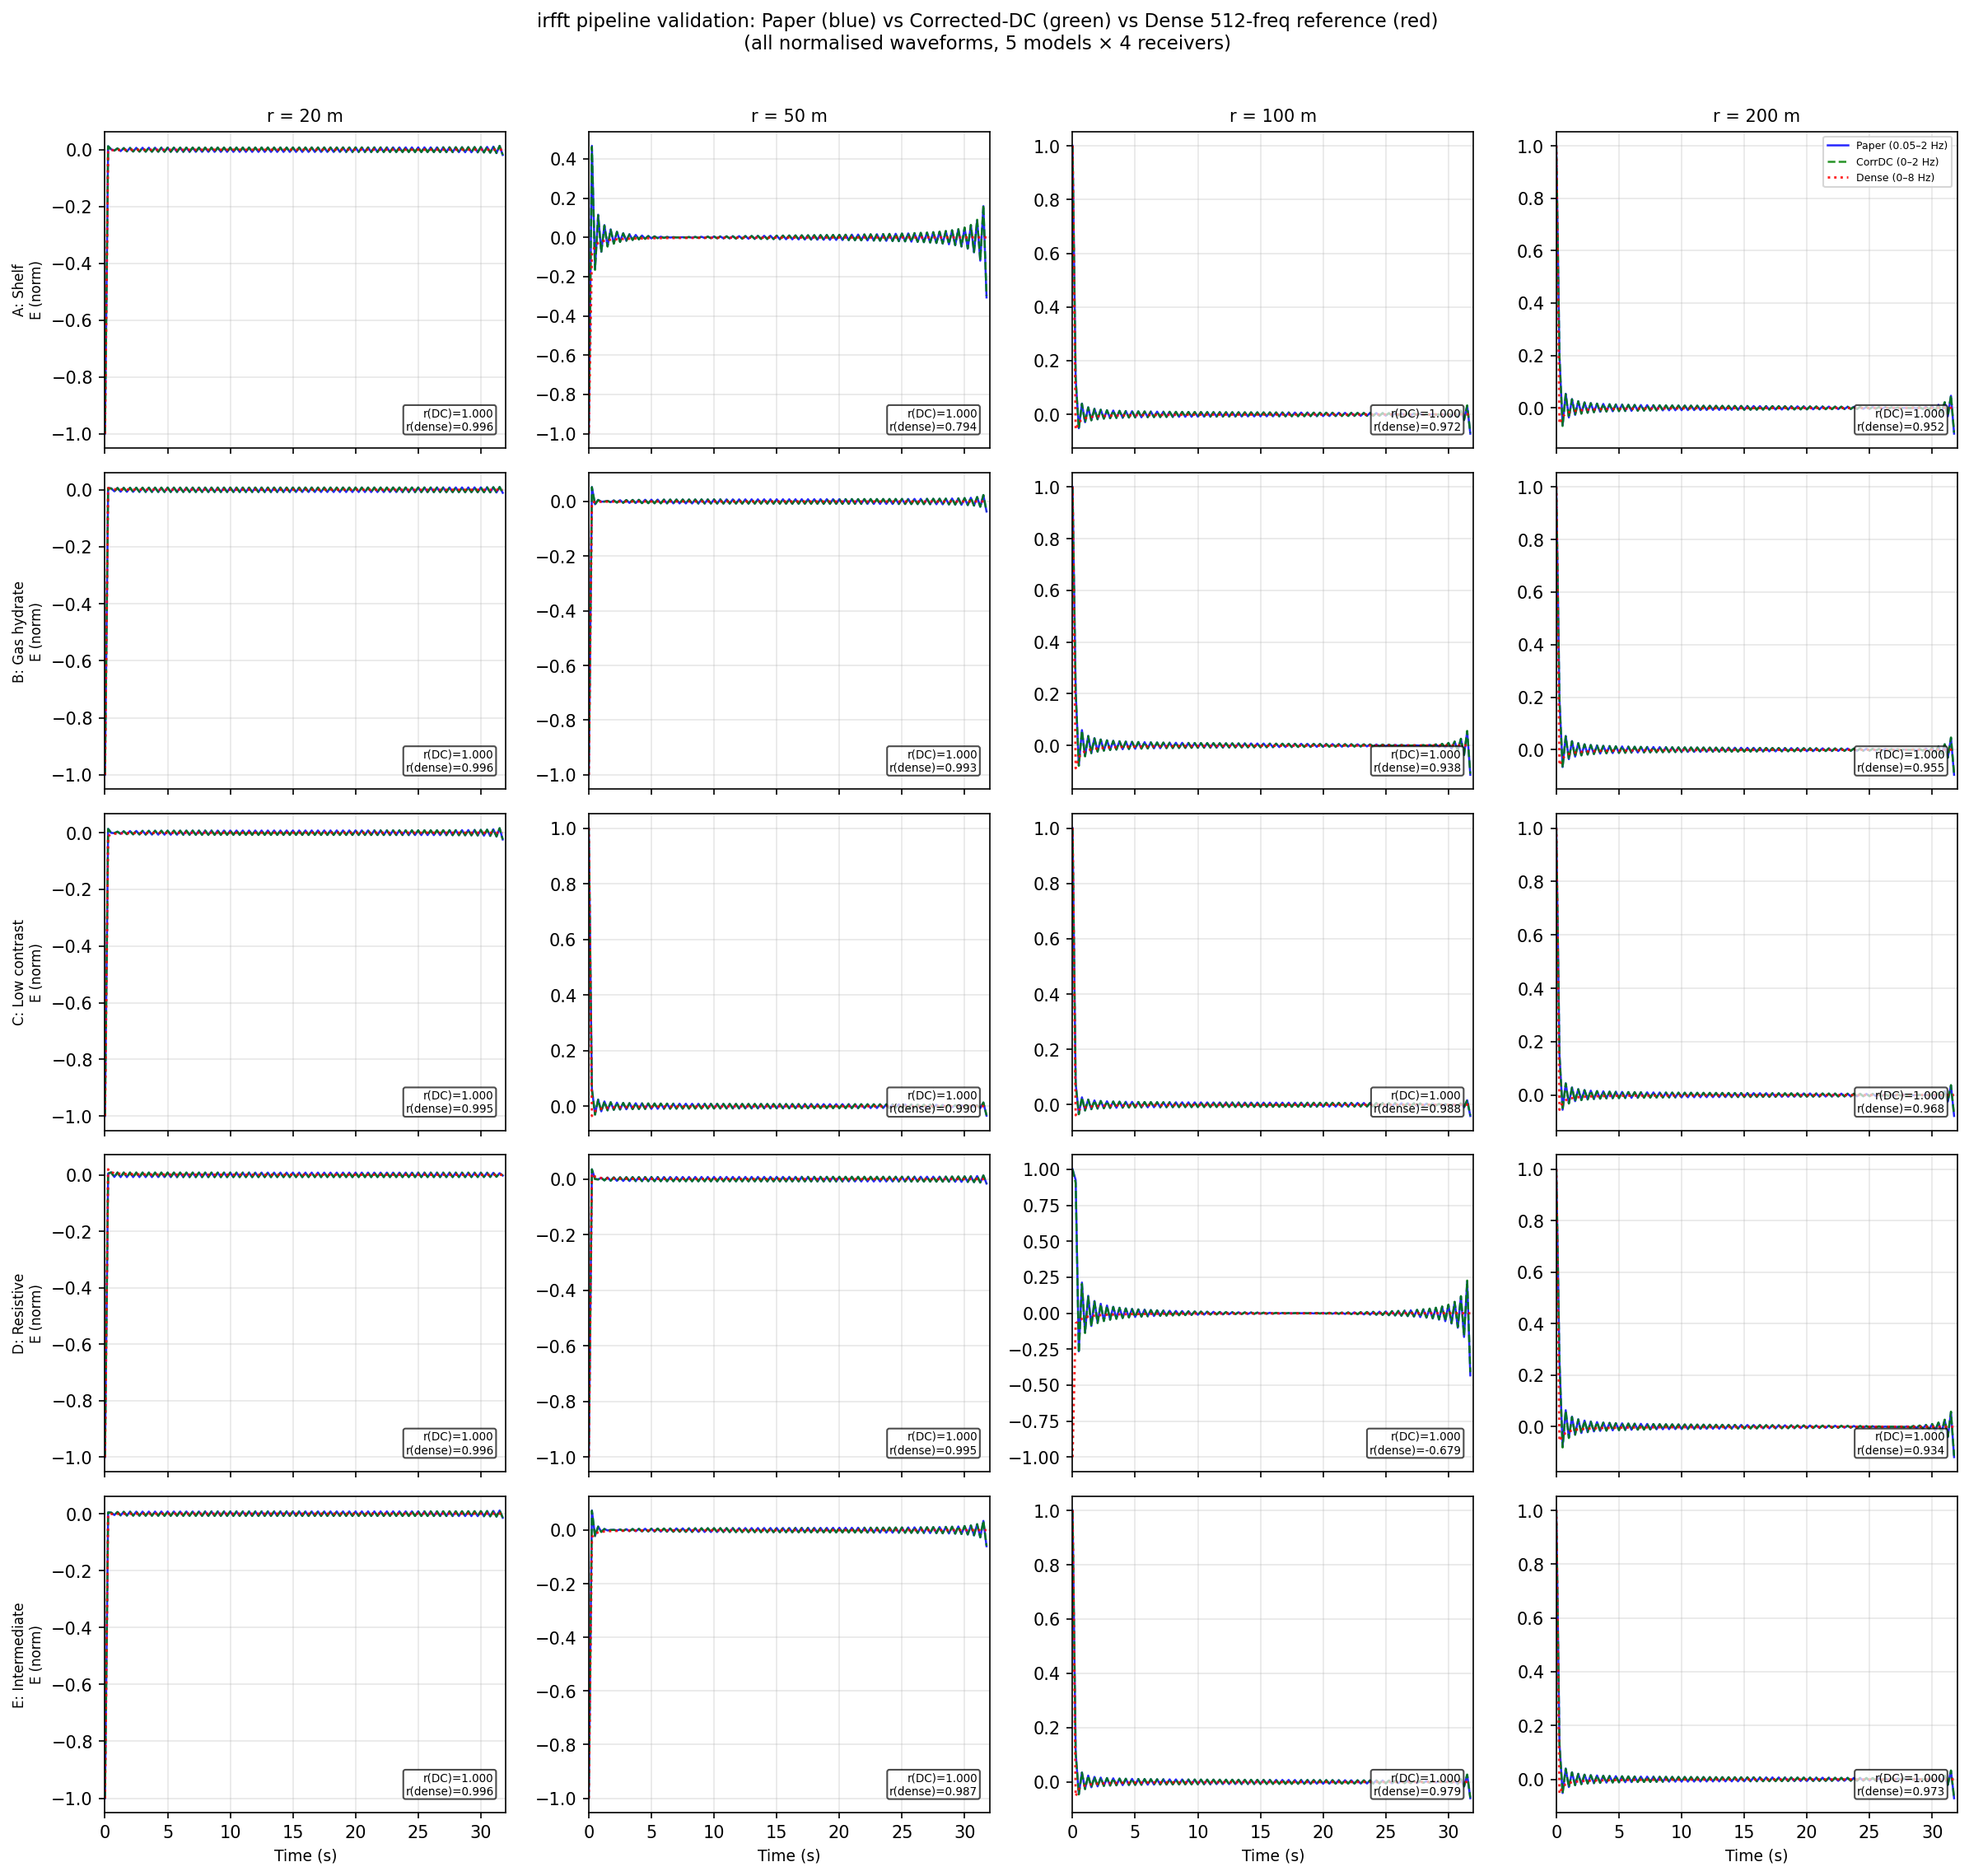
\includegraphics[width=\textwidth]{irfft_validation.png}
  \caption{Validation of the irfft synthesis pipeline.  Each panel
  overlays the normalised waveform from the paper's 64-frequency
  irfft pathway (blue solid), the corrected-DC pathway (green dashed,
  frequencies 0--2\,Hz including a near-DC proxy), and a dense
  512-frequency reference (red dotted, 0--8\,Hz).  Five
  field-representative models $\times$ four receiver offsets $= 20$
  comparisons.  The paper and corrected-DC waveforms are virtually
  identical ($r \geq 0.9998$ in all cases), confirming that the DC
  misassignment is negligible.  Differences with the dense reference
  (mean $r = 0.97$ excluding one outlier) reflect bandwidth
  truncation at 2\,Hz, not a synthesis artefact.}
  \label{fig:supp_irfft}
\end{figure}


%% ── S2: Step-Off Source Validation ───────────────────────────────────────────
\section{Step-Off Source Validation}
\label{sec:supp_stepoff}

DualTCN is trained on impulse-response waveforms.  Deployment on
field data acquired under the step-off convention requires a
pre-processing step: division by $\mathrm{i}\,2\pi f$ in the
frequency domain (or temporal integration) before the time series is
passed to the network.

To validate this pipeline, we synthesise step-off responses for the
five field-representative models and retransform them to the
impulse-response representation used by DualTCN.
Table~\ref{tab:supp_stepoff} compares the resulting predictions
(``RT'', retransformed from step-off) against predictions obtained
directly from impulse-response inputs (``Imp'').

\begin{table*}[t]
  \centering
  \footnotesize
  \caption{Step-off source validation: DualTCN predictions on
  impulse-response inputs (Imp) versus retransformed step-off inputs
  (RT) for five field-representative models.  ``Max \% diff'' is the
  largest absolute percentage difference between Imp and RT across all
  four parameters.  Units: $\sigma$ in S/m, $d$ in m.}
  \label{tab:supp_stepoff}
  \setlength{\tabcolsep}{3.5pt}
  \begin{tabular}{llrrrr@{\;\;}rrrr@{\;\;}r}
    \toprule
    & Model
      & $\hat\sigma_1^\mathrm{Imp}$ & $\hat\sigma_2^\mathrm{Imp}$
      & $\hat{d}_1^\mathrm{Imp}$ & $\hat{d}_2^\mathrm{Imp}$
      & $\hat\sigma_1^\mathrm{RT}$ & $\hat\sigma_2^\mathrm{RT}$
      & $\hat{d}_1^\mathrm{RT}$ & $\hat{d}_2^\mathrm{RT}$
      & Max \% \\
    \midrule
    A & Shelf
      & 3.04 & 0.440 & 80.3 & 36.2
      & 3.27 & 0.479 & 80.8 & 32.4 & 10.4 \\
    B & Gas hydrate
      & 3.19 & 0.055 & 97.1 & 18.0
      & 3.44 & 0.081 & 98.0 & 17.3 & 47.2 \\
    C & Low contrast
      & 2.51 & 0.714 & 58.5 & 43.2
      & 2.67 & 0.739 & 58.6 & 41.5 & 6.4 \\
    D & Resistive
      & 3.71 & 0.008 & 114.2 & 14.4
      & 3.98 & 0.017 & 115.5 & 12.0 & 117.3 \\
    E & Intermediate
      & 1.73 & 0.245 & 90.3 & 37.6
      & 1.84 & 0.276 & 90.9 & 36.3 & 12.6 \\
    \bottomrule
  \end{tabular}
\end{table*}

For three of the five models (A, C, E), the retransformation
introduces differences below 13\%, confirming that the pre-processing
pipeline is viable under typical shelf and sediment conditions.
Model~B (gas hydrate) shows a 47\% difference concentrated in
$\sigma_2$ (0.055 vs.\ 0.081\,S/m), where the low seafloor
conductivity amplifies relative sensitivity to the retransformation.
Model~D (resistive basement, $\sigma_2 = 0.008$\,S/m) is the worst
case: $\hat{\sigma}_2$ shifts from 0.008 to 0.017\,S/m (117\%
relative change), reflecting the fact that highly resistive targets
push significant spectral energy above the 2\,Hz bandwidth, and the
retransformation amplifies the resulting truncation artefact.


%% ── S3: Physical Error Conversion ────────────────────────────────────────────
\section{Physical-Unit Error Conversion}
\label{sec:supp_phys}

Table~\ref{tab:supp_phys} translates the normalised log-space RMSE
values into physical units to aid interpretability.

\begin{table*}[t]
  \centering
  \footnotesize
  \caption{DualTCN test-set RMSE converted to physical units
  (150\,000 test samples).
  $e_\mathrm{norm}$: normalised $[0,1]$ log-space RMSE.
  $e_\mathrm{log}$: RMSE in $\log_{10}$ physical units.
  $\Gamma = 10^{e_\mathrm{log}}$: geometric RMSE factor.
  ``Physical RMSE at geo-mean'': $\Gamma - 1$ applied to the
  geometric mean of the training range.}
  \label{tab:supp_phys}
  \begin{tabular}{lcccccc}
    \toprule
    Parameter & Range & Geo-mean & $e_\mathrm{norm}$ & $e_\mathrm{log}$ & $\Gamma$ & Phys.\ RMSE \\
    \midrule
    $\sigma_1$ (S\,m$^{-1}$) & 0.1--5.0 & 0.71 & 0.020 & 0.034 & 1.08 & 0.06\,S\,m$^{-1}$ \\
    $\sigma_2$ (S\,m$^{-1}$) & 0.001--1 & 0.032 & 0.092 & 0.276 & 1.89 & 0.028\,S\,m$^{-1}$ \\
    $d_1$ (m)                & 50--150 & 87 & 0.031 & 0.015 & 1.04 & 3\,m \\
    $d_2$ (m)                & 10--50  & 22 & 0.165 & 0.115 & 1.30 & 7\,m \\
    \bottomrule
  \end{tabular}
\end{table*}


%% ── S4: Full Ablation Tables ─────────────────────────────────────────────────
\section{Full Ablation Results}
\label{sec:supp_ablation}

Tables~\ref{tab:supp_rmse} and~\ref{tab:supp_r2} report normalised
RMSE, total loss, inference timing, and per-parameter $R^2$ for all
thirteen ablation variants.

\begin{table*}[t]
  \centering
  \footnotesize
  \caption{Normalised RMSE, total loss, and single-sample latency
  (A100 GPU, 1\,000 runs). Bold = best; $\dagger$ = worse than
  baseline.}
  \label{tab:supp_rmse}
  \begin{tabular}{llrcccccc}
    \toprule
    & Variant & Params & $\sigma_1$ & $\sigma_2$ & $d_1$ & $d_2$
              & Total & ms \\
    \midrule
    & PCRN        & 638K & 0.026 & 0.110 & 0.033 & 0.183
                  & 0.1032 & 2.6 \\
    P1  & 200 ep      & 638K & 0.027 & 0.102 & 0.033 & 0.184
        & 0.0932 & 2.5 \\
    P2  & +amp-ratio  & 638K & 0.027 & 0.101 & 0.034 & 0.192
        & 0.0959 & 2.6 \\
    P3$^\dagger$
        & $d_2$ wt=5  & 638K & 0.025 & 0.111 & 0.035 & 0.180
        & 0.1145 & 2.7 \\
    P4$^\dagger$
        & CrossRecv   & 576K & 0.036 & 0.179 & 0.036 & 0.259
        & 0.2469 & 2.1 \\
    P5a & TCN-only    & \textbf{201K} & 0.022 & 0.109
        & \textbf{0.031} & 0.187 & 0.1020 & 2.0 \\
    P5b$^\dagger$
        & TF-only     & 877K & 0.097 & 0.155 & 0.137 & 0.224
        & 0.2248 & 1.4 \\
    P5c$^\dagger$
        & MLP-only    & 952K & 0.091 & 0.269 & 0.082 & 0.272
        & 0.4450 & 0.5 \\
    P6$^\dagger$
        & Latent=512  & 770K & 0.027 & 0.105 & \textbf{0.031}
        & 0.208 & 0.1007 & 2.6 \\
    P7  & MultiScale  & 384K & 0.021 & 0.100 & \textbf{0.031}
        & 0.184 & 0.0931 & 3.8 \\
    P8  & TwoStage    & 401K & 0.020 & 0.098 & 0.033 & 0.185
        & 0.0892 & 3.8 \\
    P10a$^\dagger$
        & iTransf.    & 381K & 0.040 & 0.180 & 0.041 & 0.220
        & 0.2204 & 1.0 \\
    P10b$^\dagger$
        & PatchTST    & 369K & 0.050 & 0.202 & 0.050 & 0.248
        & 0.2749 & 1.1 \\
    \textbf{DualTCN}
        &             & 379K & \textbf{0.020} & \textbf{0.092}
        & \textbf{0.031} & \textbf{0.165}
        & \textbf{0.0771} & 3.5 \\
    \bottomrule
  \end{tabular}
\end{table*}

\begin{table*}[t]
  \centering
  \footnotesize
  \caption{Per-parameter $R^2$ and batch-256 throughput.
  Bold = best.}
  \label{tab:supp_r2}
  \begin{tabular}{llccccr}
    \toprule
    & Variant & $R^2_{\sigma_1}$ & $R^2_{\sigma_2}$ & $R^2_{d_1}$
              & $R^2_{d_2}$ & Throughput \\
    \midrule
    & PCRN        & 0.992 & 0.855 & 0.986 & 0.541 &  45\,K/s \\
    P1  & 200 ep      & 0.991 & 0.876 & 0.986 & 0.536
        &  44\,K/s \\
    P2  & +amp-ratio  & 0.991 & 0.877 & 0.985 & 0.496
        &  45\,K/s \\
    P3  & $d_2$ wt=5  & 0.992 & 0.853 & 0.984 & 0.560
        &  44\,K/s \\
    P4  & CrossRecv   & 0.984 & 0.615 & 0.984 & 0.082
        &  59\,K/s \\
    P5a & TCN-only    & 0.994 & 0.857 & 0.987 & 0.525
        & 127\,K/s \\
    P5b & TF-only     & 0.886 & 0.713 & 0.760 & 0.318
        &  34\,K/s \\
    P5c & MLP-only    & 0.901 & 0.133 & 0.915 & $-$0.008
        & 550\,K/s \\
    P6  & Latent=512  & 0.991 & 0.868 & 0.987 & 0.411
        &  45\,K/s \\
    P7  & MultiScale  & 0.995 & 0.879 & \textbf{0.988} & 0.539
        &  67\,K/s \\
    P8  & TwoStage    & 0.995 & 0.885 & 0.986 & 0.532
        &  67\,K/s \\
    P10a & iTransf.   & 0.980 & 0.610 & 0.979 & 0.342
        & \textbf{247\,K/s} \\
    P10b & PatchTST   & 0.970 & 0.512 & 0.968 & 0.162
        & 69\,K/s \\
    \textbf{DualTCN}
        &             & \textbf{0.995} & \textbf{0.898} & 0.987
        & \textbf{0.627} & 76\,K/s \\
    \bottomrule
  \end{tabular}
\end{table*}


%% ── S5: Transformer Discussion ───────────────────────────────────────────────
\section{Why Attention-Based Encoders Underperform}
\label{sec:supp_transformer}

Both P10a (iTransformer) and P10b (PatchTST) produce total losses
above 0.22---more than $2.8\times$ worse than DualTCN and worse than
the plain TCN-only baseline.

\subsection{Specific Configurations Tested}

We ran exploratory variants of the Transformer-only encoder (P5b)
with 1, 2, and 4 layers and 2, 4, and 8 heads (all within
$\pm 0.01$ total loss of the reported P5b).  Beyond two layers,
training instability (gradient-norm spikes) was observed.
Sinusoidal, learnable absolute, and relative (RoPE-style) positional
encodings were compared; none materially affected the final loss.
For PatchTST, patch lengths $\{8, 16, 32\}$ were tested; smaller
patches marginally improved $R^2_{\sigma_1}$ but not $R^2_{d_2}$.

\subsection{Physical Interpretation}

The core difficulty is inductive bias, not hyperparameters.  The
MCSEM transient is not exchangeable in time: the first 32 samples
encode seawater properties through a distinct diffusion regime,
while the last 64 encode the seafloor through exponential decay.
Global self-attention treats all positions as equally relevant,
which conflates these two physically separate regimes.

The iTransformer collapses each channel to a single token, discarding
temporal ordering entirely ($R^2_{d_2} = 0.342$).  PatchTST retains
locality within each patch but the channel-independent design delays
cross-receiver integration.  By contrast, DualTCN hardcodes the known
temporal structure with a separate encoder branch for the late-time
window.


%% ── S6: Full UQ Comparison ────────────────────────────────────────────────────
\section{Full Uncertainty Quantification Comparison}
\label{sec:supp_uq}

Four UQ methods are compared on 5\,000 held-out test samples:
MC-Dropout ($T = 100$ passes, $p = 0.30$), temperature-scaled
MC-Dropout, split conformal prediction ($n_\mathrm{cal} = 75{,}000$),
and a five-member deep ensemble.

MC-Dropout keeps dropout active at inference and constructs Gaussian
intervals from the predictive mean and standard deviation.
Temperature scaling learns one scalar $\tau_k$ per parameter on the
validation set to dilate the MC-Dropout variance.  Split conformal
prediction uses the empirical residual quantile to construct intervals
with provable marginal coverage.  The deep ensemble aggregates five
independently trained DualTCN models (seeds 0--4).

Table~\ref{tab:supp_uq} reports the full PICP at six nominal levels,
MPIW$_{90}$, and point-estimate RMSE.

\begin{table}[t]
  \centering
  \footnotesize
  \caption{PICP at nominal levels $\alpha \in \{50, 70, 80, 90, 95,
  99\%\}$ for four UQ methods (5\,000 held-out test samples).
  Bold = closest to nominal for $\sigma_2$ and $d_2$.}
  \label{tab:supp_uq}
  \scriptsize
  \setlength{\tabcolsep}{2pt}
  \begin{tabular}{llcccc}
    \toprule
    $\alpha$ & Method & $\sigma_1$ & $\sigma_2$ & $d_1$ & $d_2$ \\
    \midrule
    50\% & MC-Dropout      & 0.688 & 0.434 & 0.291 & 0.280 \\
         & Temp-scaled     & 0.552 & 0.609 & 0.488 & 0.585 \\
         & Split conformal & 0.504 & \textbf{0.480} & 0.489 & \textbf{0.496} \\
         & Deep ensemble   & 0.267 & 0.214 & 0.149 & 0.140 \\
    \midrule
    90\% & MC-Dropout      & \textbf{0.944} & 0.664 & 0.596 & 0.572 \\
         & Temp-scaled     & 0.863 & 0.845 & 0.905 & 0.854 \\
         & Split conformal & 0.906 & \textbf{0.900} & \textbf{0.902} & \textbf{0.905} \\
         & Deep ensemble   & 0.581 & 0.480 & 0.278 & 0.362 \\
    \midrule
    99\% & MC-Dropout      & 0.990 & 0.785 & 0.827 & 0.715 \\
         & Temp-scaled     & 0.956 & 0.940 & 0.987 & 0.947 \\
         & Split conformal & \textbf{0.993} & \textbf{0.989} & \textbf{0.990} & \textbf{0.991} \\
         & Deep ensemble   & 0.764 & 0.656 & 0.366 & 0.559 \\
    \midrule
    \multicolumn{6}{l}{\textit{MPIW$_{90}$ (normalised)}} \\
    & MC-Dropout      & 0.078 & 0.077 & 0.059 & 0.135 \\
    & Temp-scaled     & 0.055 & 0.149 & 0.112 & 0.342 \\
    & Split conformal & 0.062 & 0.306 & 0.096 & 0.500 \\
    & Deep ensemble   & 0.026 & 0.074 & 0.018 & 0.125 \\
    \bottomrule
  \end{tabular}
\end{table}


%% ── S7: Ablation Variant Descriptions ────────────────────────────────────────
\section{Ablation Variant Descriptions}
\label{sec:supp_variants}

\begin{table}[t]
  \centering
  \footnotesize
  \caption{Thirteen ablation variants and their modifications
  relative to the PCRN baseline.}
  \label{tab:supp_experiments}
  \setlength{\tabcolsep}{2pt}
  \begin{tabular}{lp{4.5cm}}
    \toprule
    ID & Modification \\
    \midrule
    P1   & Doubled training (200 epochs) \\
    P2   & Three inter-receiver log-amplitude ratios (11 ch) \\
    P3   & $d_2$ loss weight $\times 5$ \\
    P4   & Per-receiver TCN + cross-attention fusion \\
    P5a  & TCN-only encoder \\
    P5b  & Transformer-only encoder \\
    P5c  & Flat MLP encoder \\
    P6   & Latent dimension doubled to 512 \\
    P7   & Multi-scale TCN (3 dilation schedules) \\
    P8   & Two-stage cascaded prediction \\
    P10a & iTransformer \\
    P10b & PatchTST \\
    DualTCN & Late-time branch + $d_\mathrm{sf}$ head \\
    \bottomrule
  \end{tabular}
\end{table}


%% ── S8: Amplitude Perturbation Table ─────────────────────────────────────────
\section{Amplitude-Channel Perturbation Results}
\label{sec:supp_amp}

\begin{table}[t]
  \centering
  \footnotesize
  \caption{DualTCN $R^2$ under amplitude-channel perturbations
  (150\,000 test samples).  Panel~(A): random noise.
  Panel~(B): systematic bias.  Bold = clean baseline.}
  \label{tab:supp_amp}
  \setlength{\tabcolsep}{2pt}
  \begin{tabular}{l@{\;\;}ccccc}
    \toprule
    \multicolumn{6}{c}{\textbf{(A) Random noise}} \\
    $\sigma_\mathrm{amp}$ &
      $R^2_{\sigma_1}$ & $R^2_{\sigma_2}$ & $R^2_{d_1}$ & $R^2_{d_2}$ & $\bar{R}^2$ \\
    \midrule
    \textbf{0.00} & \textbf{0.995} & \textbf{0.898} & \textbf{0.987} & \textbf{0.627} & \textbf{0.877} \\
    0.01 & 0.919 & 0.380 & 0.939 & $-$0.784 & 0.363 \\
    0.02 & 0.784 & $-$0.112 & 0.803 & $-$1.465 & 0.002 \\
    0.05 & 0.368 & $-$1.149 & 0.280 & $-$2.124 & $-$0.656 \\
    0.10 & $-$0.130 & $-$1.941 & $-$0.558 & $-$2.394 & $-$1.256 \\
    0.20 & $-$0.683 & $-$2.431 & $-$1.510 & $-$2.671 & $-$1.824 \\
    \midrule
    \multicolumn{6}{c}{\textbf{(B) Systematic bias}} \\
    $\beta$ &
      $R^2_{\sigma_1}$ & $R^2_{\sigma_2}$ & $R^2_{d_1}$ & $R^2_{d_2}$ & $\bar{R}^2$ \\
    \midrule
    $-$0.20 & 0.746 & $-$0.121 & 0.980 & 0.494 & 0.525 \\
    $-$0.10 & 0.958 & 0.368 & 0.990 & 0.601 & 0.729 \\
    \textbf{0.00} & \textbf{0.995} & \textbf{0.898} & \textbf{0.987} & \textbf{0.627} & \textbf{0.877} \\
    $+$0.10 & 0.951 & 0.626 & 0.985 & 0.273 & 0.709 \\
    $+$0.20 & 0.822 & 0.351 & 0.974 & $-$0.079 & 0.517 \\
    \bottomrule
  \end{tabular}
\end{table}


%% ── S9: Full Conventional Inversion Benchmark ────────────────────────────────
\section{Full Conventional Inversion Benchmark}
\label{sec:supp_benchmark}

\begin{table*}[t]
  \centering
  \caption{DualTCN versus conventional inversion
  (same \texttt{empymod} forward operator).  All multi-start
  runs use 8 starts.  Bold = best in each column.}
  \label{tab:supp_benchmark}
  \footnotesize
  \begin{tabular}{llccccccc}
    \toprule
    & Method & $R^2_{\sigma_1}$ & $R^2_{\sigma_2}$ & $R^2_{d_1}$
             & $R^2_{d_2}$ & $\bar{R}^2$
             & s/sample & Evals \\
    \midrule
    \multicolumn{9}{l}{\textit{Untuned baselines (500 samples)}} \\
    & NLS-LM (1 start)       & 0.592 & $-$0.292 & 0.378 & $-$0.553 & 0.031 & 2.75 & 49 \\
    & NLS-LBFGSB (1 start)   & 0.465 & $-$1.077 & 0.337 & $-$0.927 & $-$0.301 & 8.01 & 291 \\
    & NLS-LM (8 starts)      & 0.938 & $-$0.330 & 0.961 & $-$1.053 & 0.129 & 12.09 & 338 \\
    & NLS-LBFGSB (8 starts)  & 0.961 & 0.179 & 0.980 & $-$0.362 & 0.439 & 73.58 & 2{,}630 \\
    \midrule
    \multicolumn{9}{l}{\textit{Occam regularised (200 samples)}} \\
    & Occam-LM ($\lambda$=0.01) & 0.730 & $-$0.385 & 0.853 & $-$1.030 & 0.042 & 14.71 & 170 \\
    \midrule
    \multicolumn{9}{l}{\textit{Improved baselines (500 samples)}} \\
    & TT-LM                  & 0.938 & $-$0.330 & 0.961 & $-$1.053 & 0.129 & 13.00 & 378 \\
    & TIK-LBFGSB             & 0.962 & 0.263 & 0.982 & $-$0.296 & 0.478 & 123.14 & 4{,}417 \\
    & WS-LM (DualTCN init)   & 0.993 & 0.689 & 0.997 & 0.343 & 0.756 & 13.22 & 380 \\
    & WS-LBFGSB (DualTCN init) & 0.993 & 0.781 & \textbf{0.998} & 0.364 & 0.784 & 92.80 & 3{,}312 \\
    \midrule
    \multicolumn{9}{l}{\textit{Neural network}} \\
    & \textbf{DualTCN}       & \textbf{0.996} & \textbf{0.884} & 0.988 & \textbf{0.578} & \textbf{0.862} & \textbf{0.0035} & 1 \\
    \bottomrule
  \end{tabular}
\end{table*}


\end{document}
